\documentclass[14pt]{extbook}
\usepackage{multicol, enumerate, enumitem, hyperref, color, soul, setspace, parskip, fancyhdr} %General Packages
\usepackage{amssymb, amsthm, amsmath, bbm, latexsym, units, mathtools} %Math Packages
\everymath{\displaystyle} %All math in Display Style
% Packages with additional options
\usepackage[headsep=0.5cm,headheight=12pt, left=1 in,right= 1 in,top= 1 in,bottom= 1 in]{geometry}
\usepackage[usenames,dvipsnames]{xcolor}
\usepackage{dashrule}  % Package to use the command below to create lines between items
\newcommand{\litem}[1]{\item#1\hspace*{-1cm}\rule{\textwidth}{0.4pt}}
\pagestyle{fancy}
\lhead{Progress Quiz 4}
\chead{}
\rhead{Version A}
\lfoot{9187-5854}
\cfoot{}
\rfoot{Spring 2021}
\begin{document}

\begin{enumerate}
\litem{
Which of the following equations \textit{could} be of the graph presented below?
\begin{center}
    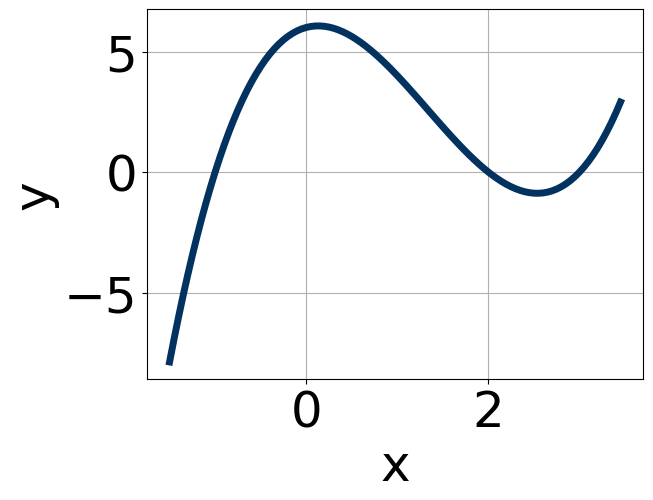
\includegraphics[width=0.5\textwidth]{../Figures/polyGraphToFunctionCopyA.png}
\end{center}
\begin{enumerate}[label=\Alph*.]
\item \( 12x^{5} (x - 3)^{6} (x - 1)^{8} \)
\item \( 3x^{10} (x - 3)^{10} (x - 1)^{7} \)
\item \( -16x^{6} (x - 3)^{6} (x - 1)^{6} \)
\item \( 10x^{7} (x - 3)^{8} (x - 1)^{9} \)
\item \( -4x^{4} (x - 3)^{6} (x - 1)^{9} \)

\end{enumerate} }
\litem{
Describe the end behavior of the polynomial below.\[ f(x) = -8(x - 6)^{4}(x + 6)^{5}(x - 3)^{3}(x + 3)^{5} \]\begin{enumerate}[label=\Alph*.]
\begin{multicols}{2}\item 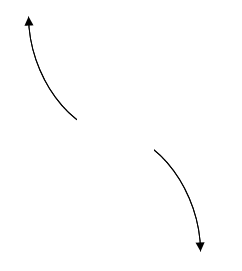
\includegraphics[width = 0.3\textwidth]{../Figures/polyEndBehaviorCopyAA.png}\item 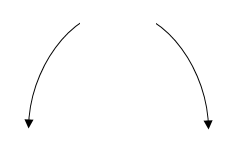
\includegraphics[width = 0.3\textwidth]{../Figures/polyEndBehaviorCopyBA.png}\item 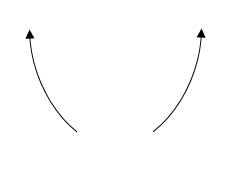
\includegraphics[width = 0.3\textwidth]{../Figures/polyEndBehaviorCopyCA.png}\item 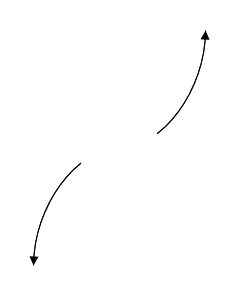
\includegraphics[width = 0.3\textwidth]{../Figures/polyEndBehaviorCopyDA.png}\end{multicols}\item None of the above.
\end{enumerate} }
\litem{
Construct the lowest-degree polynomial given the zeros below. Then, choose the intervals that contain the coefficients of the polynomial in the form $ax^3+bx^2+cx+d$.\[ \frac{-3}{2}, 3, \text{ and } \frac{2}{5} \]\begin{enumerate}[label=\Alph*.]
\item \( a \in [9, 13], b \in [-20, -16], c \in [-42, -33], \text{ and } d \in [-19, -12] \)
\item \( a \in [9, 13], b \in [9, 17], c \in [-51, -46], \text{ and } d \in [13, 22] \)
\item \( a \in [9, 13], b \in [-20, -16], c \in [-42, -33], \text{ and } d \in [13, 22] \)
\item \( a \in [9, 13], b \in [-50, -48], c \in [63, 65], \text{ and } d \in [-19, -12] \)
\item \( a \in [9, 13], b \in [19, 25], c \in [-42, -33], \text{ and } d \in [-19, -12] \)

\end{enumerate} }
\litem{
Describe the zero behavior of the zero $x = -8$ of the polynomial below.\[ f(x) = -4(x + 8)^{5}(x - 8)^{10}(x + 2)^{8}(x - 2)^{12} \]\begin{enumerate}[label=\Alph*.]
\begin{multicols}{2}\item 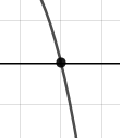
\includegraphics[width = 0.3\textwidth]{../Figures/polyZeroBehaviorAA.png}\item 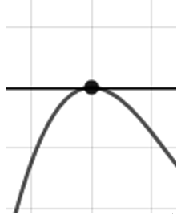
\includegraphics[width = 0.3\textwidth]{../Figures/polyZeroBehaviorBA.png}\item 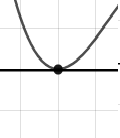
\includegraphics[width = 0.3\textwidth]{../Figures/polyZeroBehaviorCA.png}\item 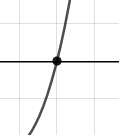
\includegraphics[width = 0.3\textwidth]{../Figures/polyZeroBehaviorDA.png}\end{multicols}\item None of the above.
\end{enumerate} }
\litem{
Describe the end behavior of the polynomial below.\[ f(x) = -2(x - 4)^{5}(x + 4)^{8}(x + 6)^{5}(x - 6)^{5} \]\begin{enumerate}[label=\Alph*.]
\begin{multicols}{2}\item 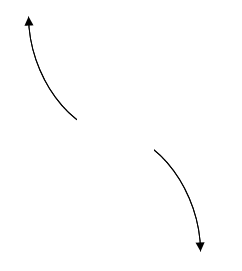
\includegraphics[width = 0.3\textwidth]{../Figures/polyEndBehaviorAA.png}\item 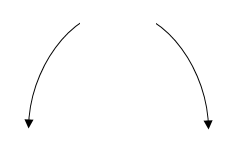
\includegraphics[width = 0.3\textwidth]{../Figures/polyEndBehaviorBA.png}\item 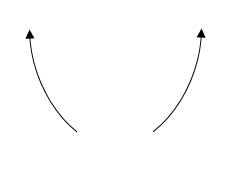
\includegraphics[width = 0.3\textwidth]{../Figures/polyEndBehaviorCA.png}\item 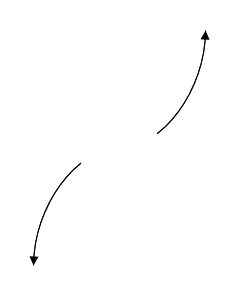
\includegraphics[width = 0.3\textwidth]{../Figures/polyEndBehaviorDA.png}\end{multicols}\item None of the above.
\end{enumerate} }
\litem{
Construct the lowest-degree polynomial given the zeros below. Then, choose the intervals that contain the coefficients of the polynomial in the form $x^3+bx^2+cx+d$.\[ 4 - 5 i \text{ and } 2 \]\begin{enumerate}[label=\Alph*.]
\item \( b \in [-5, 5], c \in [-5, 4], \text{ and } d \in [-10, -7] \)
\item \( b \in [-11, -4], c \in [54, 62], \text{ and } d \in [-87, -81] \)
\item \( b \in [-5, 5], c \in [-10, 1], \text{ and } d \in [7, 9] \)
\item \( b \in [9, 17], c \in [54, 62], \text{ and } d \in [79, 83] \)
\item \( \text{None of the above.} \)

\end{enumerate} }
\litem{
Which of the following equations \textit{could} be of the graph presented below?
\begin{center}
    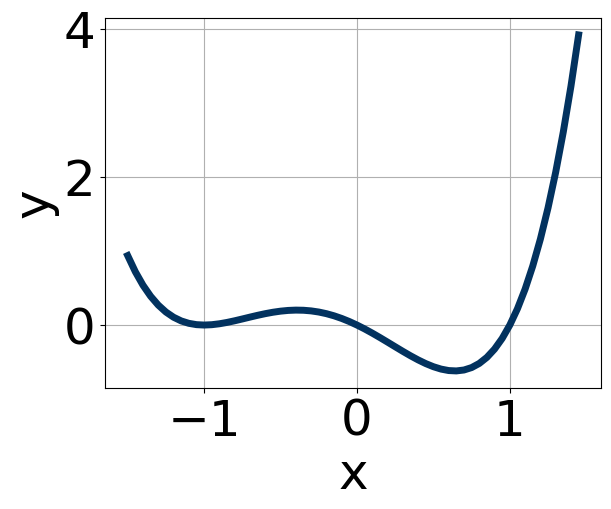
\includegraphics[width=0.5\textwidth]{../Figures/polyGraphToFunctionA.png}
\end{center}
\begin{enumerate}[label=\Alph*.]
\item \( -13x^{11} (x - 1)^{7} (x + 2)^{5} \)
\item \( 13x^{9} (x - 1)^{8} (x + 2)^{9} \)
\item \( 13x^{11} (x - 1)^{11} (x + 2)^{9} \)
\item \( -18x^{7} (x - 1)^{8} (x + 2)^{7} \)
\item \( 18x^{4} (x - 1)^{10} (x + 2)^{11} \)

\end{enumerate} }
\litem{
Construct the lowest-degree polynomial given the zeros below. Then, choose the intervals that contain the coefficients of the polynomial in the form $x^3+bx^2+cx+d$.\[ -3 + 5 i \text{ and } 4 \]\begin{enumerate}[label=\Alph*.]
\item \( b \in [-4.9, -0.1], c \in [9, 18], \text{ and } d \in [134, 142] \)
\item \( b \in [-0.2, 1.3], c \in [-1, 9], \text{ and } d \in [-14, -5] \)
\item \( b \in [1.2, 8], c \in [9, 18], \text{ and } d \in [-137, -135] \)
\item \( b \in [-0.2, 1.3], c \in [-14, -8], \text{ and } d \in [20, 25] \)
\item \( \text{None of the above.} \)

\end{enumerate} }
\litem{
Describe the zero behavior of the zero $x = -3$ of the polynomial below.\[ f(x) = -9(x - 3)^{4}(x + 3)^{5}(x - 8)^{4}(x + 8)^{8} \]\begin{enumerate}[label=\Alph*.]
\begin{multicols}{2}\item 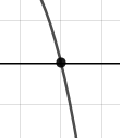
\includegraphics[width = 0.3\textwidth]{../Figures/polyZeroBehaviorCopyAA.png}\item 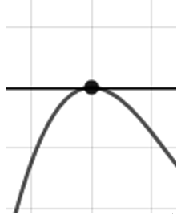
\includegraphics[width = 0.3\textwidth]{../Figures/polyZeroBehaviorCopyBA.png}\item 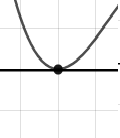
\includegraphics[width = 0.3\textwidth]{../Figures/polyZeroBehaviorCopyCA.png}\item 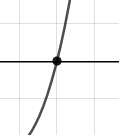
\includegraphics[width = 0.3\textwidth]{../Figures/polyZeroBehaviorCopyDA.png}\end{multicols}\item None of the above.
\end{enumerate} }
\litem{
Construct the lowest-degree polynomial given the zeros below. Then, choose the intervals that contain the coefficients of the polynomial in the form $ax^3+bx^2+cx+d$.\[ \frac{5}{4}, \frac{-1}{3}, \text{ and } \frac{-7}{3} \]\begin{enumerate}[label=\Alph*.]
\item \( a \in [31, 37], b \in [51, 53], c \in [-96, -85], \text{ and } d \in [27, 44] \)
\item \( a \in [31, 37], b \in [-55, -44], c \in [-96, -85], \text{ and } d \in [27, 44] \)
\item \( a \in [31, 37], b \in [51, 53], c \in [-96, -85], \text{ and } d \in [-41, -27] \)
\item \( a \in [31, 37], b \in [117, 121], c \in [62, 71], \text{ and } d \in [-41, -27] \)
\item \( a \in [31, 37], b \in [140, 143], c \in [142, 157], \text{ and } d \in [27, 44] \)

\end{enumerate} }
\end{enumerate}

\end{document}